
\begin{minipage}[T]{.45\textwidth}
  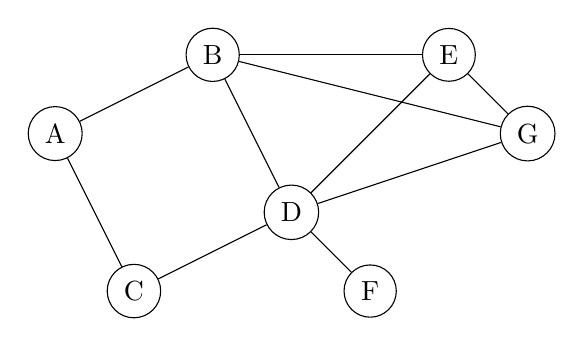
\begin{tikzpicture}[scale=1]
    \node[draw, circle] (A) at (0, 2) {A};
    \node[draw, circle] (B) at (2, 3) {B};
    \node[draw, circle] (C) at (1, 0) {C};
    \node[draw, circle] (D) at (3, 1) {D};
    \node[draw, circle] (E) at (5, 3) {E};
    \node[draw, circle] (F) at (4, 0) {F};
    \node[draw, circle] (G) at (6, 2) {G};
    \draw (A) -- (B);
    \draw (A) -- (C);
    \draw (B) -- (D);
    \draw (B) -- (E);
    \draw (B) -- (G);
    \draw (C) -- (D);
    \draw (D) -- (E);
    \draw (D) -- (F);
    \draw (D) -- (G);
    \draw (E) -- (G);
  \end{tikzpicture}
\end{minipage}
%
\begin{minipage}[T]{.45\textwidth}
  \begin{lstlisting}
    mapa = {
      'A': {'B', 'C'},
      'B': {'A', 'D', 'E', 'G'},
      'C': {'A', 'D'},
      'D': {'B', 'C', 'E', 'G', 'F'},
      'E': {'B', 'D', 'G'},
      'F': {'D'},
      'G': {'E', 'B', 'D'},
    }
  \end{lstlisting}
\end{minipage}

\begin{enumerate}
  \item
    Escriba la función \li!son_ciudades_vecinas(mapa, p, q)!
    que retorne un valor booleano
    indicando si las ciudades \li!p! y \li!q!
    son o no vecinas en el \li!mapa!.

\end{enumerate}

